\documentclass[11pt,conference]{IEEEtran}
\IEEEoverridecommandlockouts
% The preceding line is only needed to identify funding in the first footnote. If that is unneeded, please comment it out.
\usepackage{cite}
\usepackage{amsmath,amssymb,amsfonts}
\usepackage{graphicx}
\usepackage{textcomp}
\usepackage{xcolor}
\def\BibTeX{{\rm B\kern-.05em{\sc i\kern-.025em b}\kern-.08em
T\kern-.1667em\lower.7ex\hbox{E}\kern-.125emX}}
\begin{document}

\title{Using Supervised Learning To Solve Text-Based CAPTCHAs\\
}

\author{\IEEEauthorblockN{Turhan Kimbrough}
\IEEEauthorblockA{\textit{Department of Computer Science} \\
\textit{Towson University}\\
Towson, Maryland\\
tkimbr1@students.towson.edu}
}

\maketitle

\begin{abstract}
    CAPTCHA is an acronym for the "Completely Automated Public Turing test
    to tell Computers and Humans Apart". It is a mechanism which is used to
    distinguish real human users from bots. CAPTCHAs come in a variety of forms,
    including the deciphering of obfuscated text, transcribing of audio messages,
    tracking mouse movement, and more. This research will focus on automating the
    process of deciphering text-based CAPTCHAs using machine learning
    techniques. Specifically, supervised learning is used to develop
    neural networks capable of 100\% accuracy for certain datasets. The goal of
    this research is to demonstrate the weaknesses associated with text-based
    CAPTCHA mechanisms, especially with the prevalence of machine learning
    tools.
\end{abstract}

\begin{IEEEkeywords}
    machine learning, neural networks, supervised training, CAPTCHA
\end{IEEEkeywords}

\section{Introduction}
CAPTCHA is an acronym for the "\textbf{C}ompletely \textbf{A}utomated
\textbf{P}ublic \textbf{T}uring test to tell
\textbf{C}omputers and \textbf{H}umans \textbf{A}part", which is a
challenge-response test used in computing services to verify that user is a
human. The premise of a CAPTCHA is to provide a test which is relatively easy
for a human to solve, but difficult for bots. This is one of many 
mechanisms used to combat against the growing usage of malicious software
automation. Due to the ubiquity of automation software, cybercriminals have
been able to easily create bots to perform malicious acts. These acts include
denial-of-service attacks, autonomous social media communication agents,
scalping scarce merchandise, and more.

Due to the wide availability of CAPTCHA-generating software, they have become a popular
mechanism to integrate into websites. In particular, text-based CAPTCHAs are
often available as a low-cost and simple solution. Text-based CAPTCHAs
typically consist of alphanumeric characters in an image, which has been
manipulated to prevent it from being easily parsed by a machine. 

\begin{figure}[htbp]
    \centerline{\includegraphics{numeric-captcha.png}}
    \centerline{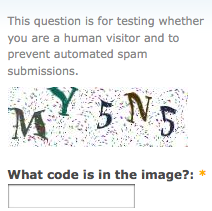
\includegraphics{alphanumeric-captcha.png}}
    \caption{Example of a text-based CAPTCHA.}
    \label{figure}
\end{figure}

While this mechanism can mitigate the majority of software bots, it is not
effective against bots utilizing machine learning technology. This research
paper demonstrates that a machine learning agent is capable of solving CAPTCHAs
with the use of an open-source framework, several
libraries, and supervised learning. The goal of this research is to
highlight the vulnerabilities which are present in simple CAPTCHA mechanisms.


\section{Methodology}

\section{Challenges}

\section{Key Contributions}

\section{Results}

\section{Background/Related Work}

\section{Future Work}


\begin{thebibliography}{00}
    \bibitem{b1} G. Eason, B. Noble, and I. N. Sneddon, ``On certain integrals of Lipschitz-Hankel type involving products of Bessel functions,'' Phil. Trans. Roy. Soc. London, vol. A247, pp. 529--551, April 1955.
    \bibitem{b2} J. Clerk Maxwell, A Treatise on Electricity and Magnetism, 3rd ed., vol. 2. Oxford: Clarendon, 1892, pp.68--73.
    \bibitem{b3} I. S. Jacobs and C. P. Bean, ``Fine particles, thin films and exchange anisotropy,'' in Magnetism, vol. III, G. T. Rado and H. Suhl, Eds. New York: Academic, 1963, pp. 271--350.
    \bibitem{b4} K. Elissa, ``Title of paper if known,'' unpublished.
    \bibitem{b5} R. Nicole, ``Title of paper with only first word capitalized,'' J. Name Stand. Abbrev., in press.
    \bibitem{b6} Y. Yorozu, M. Hirano, K. Oka, and Y. Tagawa, ``Electron spectroscopy studies on magneto-optical media and plastic substrate interface,'' IEEE Transl. J. Magn. Japan, vol. 2, pp. 740--741, August 1987 [Digests 9th Annual Conf. Magnetics Japan, p. 301, 1982].
    \bibitem{b7} M. Young, The Technical Writer's Handbook. Mill Valley, CA: University Science, 1989.
\end{thebibliography}
\vspace{12pt}
\color{red}
IEEE conference templates contain guidance text for composing and formatting conference papers. Please ensure that all template text is removed from your conference paper prior to submission to the conference. Failure to remove the template text from your paper may result in your paper not being published.

\end{document}
